\chapter{実装}
\label{chap:implementation}

本章では、第3章で述べたシステムの設計を受け、『わかるらんど』の実装について述べる。

\newpage

\section{アプリケーション構成}

『わかるらんど』のクライアントはHTML/CSS/JavaScriptで実装されており,
通常のブラウザ上のWebアプリケーションとして動作する.
サーバは,並列計算プリミティブである
\textit{Linda}\cite{Carriero:1989:LC:63334.63337}を
Webサーバ上に実装した
\textit{WebLinda}\cite{shokai_furnitue}\footnote{https://github.com/node-linda/linda}を用いて実装している.

\section{Linda}

\textit{Linda}は,
複数のプロセスで共有される空間を用いて
プロセス間通信やデータ共有をサポートする
分散並列処理を行うためのモデルである.
プロセスが共有する空間は\textbf{タプル空間} (Tuple Space) と呼ばれ,
タプル空間内のデータ (Tuple) を使って通信やデータ共有を行う (図\ref{linda}).
\textit{Linda}のモデルはきわめて単純であるが,
各クライアントやデバイス間で直接送信をする処理を記述する必要がなく,
柔軟で強力なプロセス間通信を容易に記述することができる.

\begin{figure}[h]
\centering
\fbox{
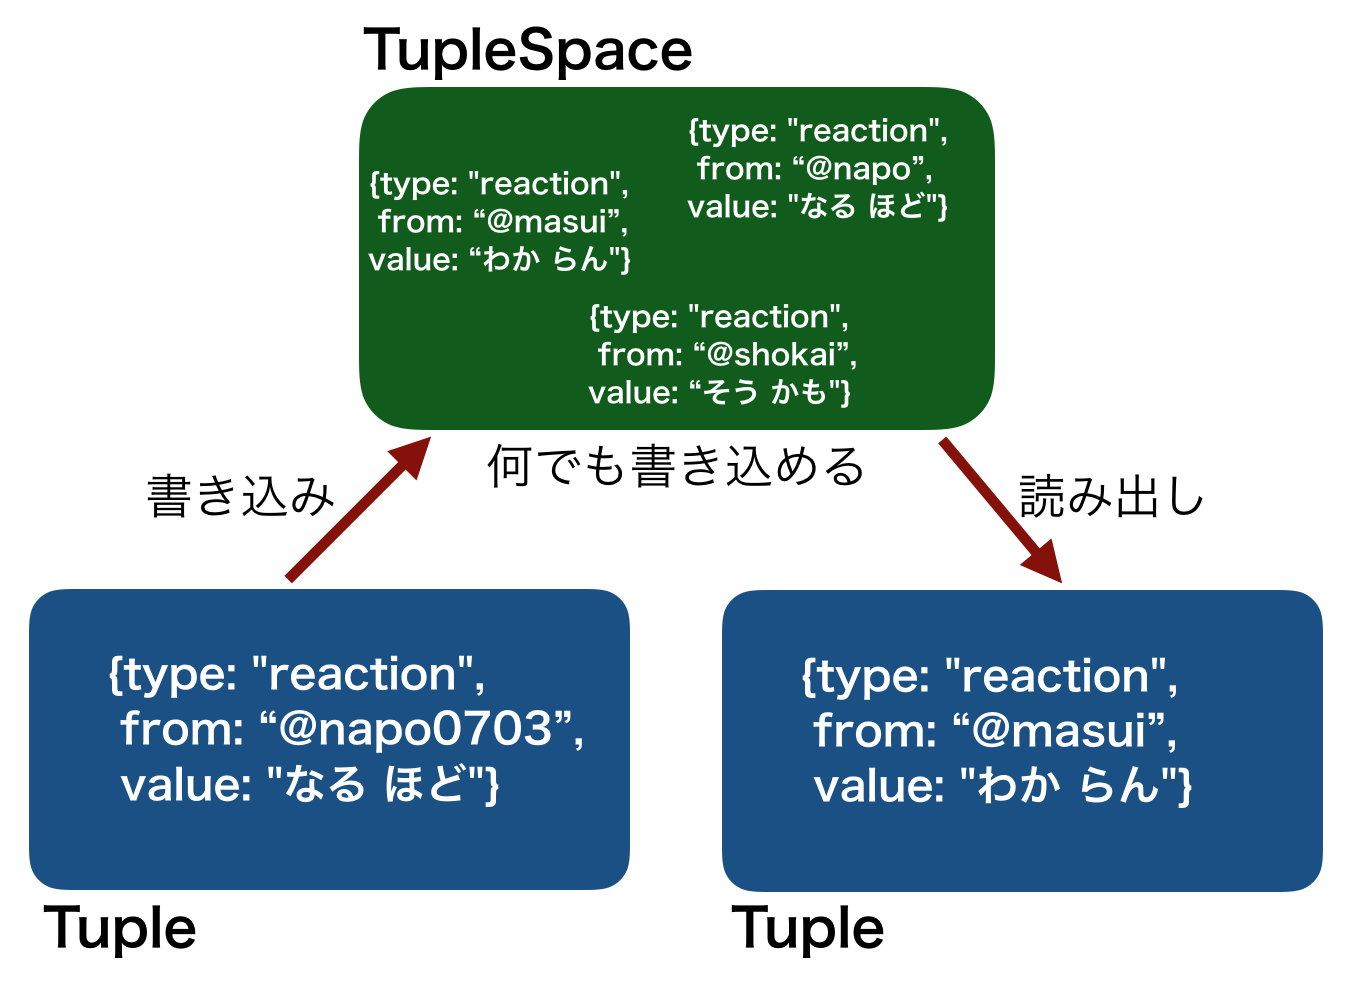
\includegraphics[width=9cm]{images/linda.png}
}
\caption{タプル空間を利用したプロセス間通信}
\label{linda}
\end{figure}

\section{WebLinda}

\textit{WebLinda}は,橋本翔氏が開発したオープンソースソフトウェアで,
% \footnote{http://shokai.org}
Node.js\footnote{https://nodejs.org}の
WebSocketライブラリ「Socket.IO\footnote{http://socket.io}」で
実装されている.
\textit{WebLinda}は通常のWebサーバ上に実装されているため,
HTTP通信をサポートする様々な環境やプログラミング言語で利用可能である.
それゆえ,Arduino\footnote{https://www.arduino.cc}や
Raspberry Pi\footnote{https://www.raspberrypi.org}
などといった各種のIoT機器との連携も容易である.

\textit{WebLinda}は,\texttt{write}, \texttt{read}, \texttt{take}, \texttt{watch}という
4つの基本操作によってプロセス間通信を行う.

\vspace{2mm}
\begin{description}
\item[\texttt{write}]\mbox{}\\
新しいデータオブジェクト(タプル)を生成し共有空間(タプル空間)に書き込む.
\item[\texttt{read}]\mbox{}\\
タプル空間からタプルを読み出す.
\item[\texttt{take}]\mbox{}\\
\texttt{read}しつつ,読み出したタプルをタプル空間から削除する.
\item[\texttt{watch}]\mbox{}\\
タプル空間を監視し,一致するタプルが
\texttt{write}された瞬間に読み出す.
\end{description}

\section{WebLindaによる『わかるらんど』の実装}

『わかるらんど』での\textit{WebLinda}実装について述べる.
ユーザのリアクションを投稿/表示する際には,
センサと『わかるらんど』の間で

\begin{lstlisting}
{
    type: "reaction",
    from: "@napo0703",
    display: "60",
    value: "なる ほど"
}
\end{lstlisting}
というようなタプルをやりとりしている.

センサやWebのデータを投稿/表示する際には,
\begin{lstlisting}
{
    type: "data",
    from: "明るさ",
    display: "60",
    value: "500",
    background: "http://masuilab.org/image.jpg"
}
\end{lstlisting}
というようなタプルをやりとりしている.

\vspace{2mm}
\begin{description}
\item[\texttt{type}]\mbox{}\\
ユーザのリアクションの場合は\texttt{reaction},
データの場合は\texttt{data}を値にする.

\item[\texttt{from}]\mbox{}\\
投稿元を表す値.

\item[\texttt{display}]\mbox{}\\
リアクションやデータの表示時間.単位は秒.リアクションやデータが表示されてからこの秒数が経過すると,自動的に取り下げられ表示されなくなる.
%20〜86400の間で指定が可能.

\item[\texttt{value}]\mbox{}\\
リアクションの場合,この値がWebにある画像ファイルのURLだった時は,その画像を投稿者のセルにオーバーレイ表示する.URLでない文字列の場合は,その文字列を投稿者のセルにオーバーレイ表示する.
データの場合,この値がそのままセルの下部に表示される.

\item[\texttt{background}(データのみ)]\mbox{}\\
データセルの背景画像のURL.そのデータが何を表すものなのか分かる画像を表示する.
\end{description}
\vspace{4mm}

以下は,ボタンを押した際に『わかるらんど』にユーザ「@napo0703」として「なる ほど」という「リアクション」を「20秒」表示するタプルを書き込むJavaScriptプログラムの例である.

\vspace{2mm}
\begin{lstlisting}
// Lindaに接続
const url = "http://linda.masuilab.org";
const socket = SocketIO(url);
const linda = new Linda().connect(socket);
const ts = linda.tuplespace("masuilab");

// ボタンを押したらタプル空間にデータ書き込み
const button = $("button").click(function () {
  ts.write({
    type: "reaction",
    from: "@napo0703",
    display: "20",
    value: "http://masuilab.org/image.jpg",
  };
});
\end{lstlisting}
以下は,先程のプログラムで書き込まれるタプルと合致する
\texttt{{from: "@napo0703", type: "reaction"}}を含むタプルが書き込まれた場合に
リアクションを表示するJavaScriptプログラムの例である.
\vspace{2mm}
\begin{lstlisting}
// Lindaに接続
const url = "http://linda.masuilab.org";
const socket = SocketIO(url);
const linda = new Linda().connect(socket);
const ts = linda.tuplespace("masuilab");
// 合致するタプルが書き込まれたら画像を変える
ts.watch({
    from: "@napo0703",
    type: "reaction"
    }, function (tuple) {
  $("img").attr("src", tuple.data.value);
};
\end{lstlisting}
\vspace{4mm}
以下は現在の江ノ島の風向と風速をタプル空間に書き込むRubyプログラムである.
Nokogiri\footnote{http://www.nokogiri.org}というライブラリで
Webページから必要な情報をスクレイピングしてタプル空間に書き込んでいる.
\vspace{2mm}
\begin{lstlisting}
url = 'http://linda.masuilab.org'
linda = Linda::SocketIO::Client.connect url
ts = linda.tuplespace('masuilab')
ts.on :connect do
  // Nokogiriでスクレイピング
  web = 'http://www.s-n-p.jp/kishou.htm'
  doc = Nokogiri::HTML(open(web))
  // 必要な情報を取得
  tds = doc.xpath('//td')
  as = tds[16].xpath('.//b').text.sub(/[^\d\.].*$/,'')
  ad = tds[19].xpath('.//b').text
  // タプル空間に書き込み
  ts.write(
      where: 'enoshima',
      type: 'data',
      name: 'wind',
      value: ad + as.to_f + ‘m/s')
end
\end{lstlisting}